% answers.tex —— 2007 年·普通高等学校招生考试·江西卷·文科 · 参考答案与详细解析片段
% 由 tools/generate_projects.py 依来源总账自 2007/2007_数学真题_江西文_试题.md + 2007/2007_数学真题_江西文_解析正文.md + 2007/2007_数学真题_江西文_答案要点.md 生成，勿手改（改源 MD 后重跑）


\begin{gktip}
固定候选 PDF 仅含题面，无答案、解析和评分标准，原卷亦未标注分值；以下为非官方编者独立推导，官方答案字段为空。来源发布者、出版者、版次与官方身份均未核。
\end{gktip}

\begin{answer}
\gksolhead{1}{}

\textbf{题目}：

若集合 $M=\{0,1\}$，$I=\{0,1,2,3,4,5\}$，则 $\complement_IM$ 为（　）

（A）$\{0,1\}$

（B）$\{2,3,4,5\}$

（C）$\{0,2,3,4,5\}$

（D）$\{1,2,3,4,5\}$

\Needspace{4\baselineskip}
\textbf{解析}

$\complement_IM$ 为 $I$ 中不属于 $M$ 的元素，即 $\{2,3,4,5\}$。

\gkanswer{答案：B。}

\end{answer}
\begin{answer}
\gksolhead{2}{}

\textbf{题目}：

函数 $y=5\tan(2x+1)$ 的最小正周期为（　）

（A）$\dfrac{\pi}{4}$

（B）$\dfrac{\pi}{2}$

（C）$\pi$

（D）$2\pi$

\Needspace{4\baselineskip}
\textbf{解析}

$y=5\tan(2x+1)$ 的最小正周期为 $\dfrac{\pi}{2}$。

\gkanswer{答案：B。}

\end{answer}
\begin{answer}
\gksolhead{3}{}

\textbf{题目}：

函数 $f(x)=\lg\dfrac{1-x}{x-4}$ 的定义域为（　）

（A）$(1,4)$

（B）$[1,4)$

（C）$(-\infty,1)\cup(4,+\infty)$

（D）$(-\infty,1]\cup(4,+\infty)$

\Needspace{4\baselineskip}
\textbf{解析}

\Needspace{5\baselineskip}
真数大于零：

\nopagebreak[4]
\[\frac{1-x}{x-4}>0\ \Leftrightarrow\ (1-x)(x-4)>0.\]

\Needspace{5\baselineskip}
两根为 $1$，$4$，二次式在两根之间为正，故

\nopagebreak[4]
\[1<x<4.\]

\gkanswer{答案：A。}

\end{answer}
\begin{answer}
\gksolhead{4}{}

\textbf{题目}：

若 $\tan\alpha=3$，$\tan\beta=\dfrac43$，则 $\tan(\alpha-\beta)$ 等于（　）

（A）$-3$

（B）$-\dfrac13$

（C）$3$

（D）$\dfrac13$

\Needspace{4\baselineskip}
\textbf{解析}

\nopagebreak[4]
\[\tan(\alpha-\beta)=\frac{\tan\alpha-\tan\beta}{1+\tan\alpha\tan\beta}=\frac{3-\frac43}{1+3\times\frac43}=\frac{\frac53}{5}=\frac13.\]

\gkanswer{答案：D。}

\end{answer}
\begin{answer}
\gksolhead{5}{}

\textbf{题目}：

设 $(x^2+1)(2x+1)^9=a_0+a_1(x+2)+a_2(x+2)^2+\cdots+a_{11}(x+2)^{11}$，则 $a_0+a_1+a_2+\cdots+a_{11}$ 的值为（　）

（A）$-2$

（B）$-1$

（C）$1$

（D）$2$

\Needspace{4\baselineskip}
\textbf{解析}

\Needspace{5\baselineskip}
令 $x+2=1$，即 $x=-1$，则

\nopagebreak[4]
\[a_0+a_1+\cdots+a_{11}=((-1)^2+1)(2(-1)+1)^9=2\times(-1)^9=-2.\]

\gkanswer{答案：A。}

\end{answer}
\begin{answer}
\gksolhead{6}{}

\textbf{题目}：

一袋中装有大小相同，编号分别为 $1$，$2$，$3$，$4$，$5$，$6$，$7$，$8$ 的八个球，从中有放回地每次取一个球，共取 $2$ 次，则取得两个球的编号和不小于 $15$ 的概率为（　）

（A）$\dfrac1{32}$

（B）$\dfrac1{64}$

（C）$\dfrac3{32}$

（D）$\dfrac3{64}$

\Needspace{4\baselineskip}
\textbf{解析}

\Needspace{5\baselineskip}
每次有 $8$ 种取法，共 $64$ 个等可能结果。两球编号和不少于 $15$ 的有

\nopagebreak[4]
\[(7,8),\ (8,7),\ (8,8),\]

共 $3$ 个，故概率为 $\dfrac3{64}$。

\gkanswer{答案：D。}

\end{answer}
\begin{answer}
\gksolhead{7}{}

\textbf{题目}：

连接抛物线 $x^2=4y$ 的焦点 $F$ 与点 $M(1,0)$ 所得的线段与抛物线交于点 $A$，设点 $O$ 为坐标原点，则三角形 $OAM$ 的面积为（　）

（A）$-1+\sqrt2$

（B）$\dfrac32-\sqrt2$

（C）$1+\sqrt2$

（D）$\dfrac32+\sqrt2$

\Needspace{4\baselineskip}
\textbf{解析}

\Needspace{5\baselineskip}
抛物线 $x^2=4y$ 的焦点为 $F(0,1)$。直线 $FM$ 过 $(0,1)$，$(1,0)$：

\nopagebreak[4]
\[y=1-x.\]

\Needspace{5\baselineskip}
与 $x^2=4y$ 联立：

\nopagebreak[4]
\[x^2=4(1-x)\ \Rightarrow\ x^2+4x-4=0.\]

\Needspace{5\baselineskip}
线段 $FM$ 上的交点满足 $0\leqslant x\leqslant1$，故

\nopagebreak[4]
\[x_A=-2+2\sqrt2,\]

\nopagebreak[4]
\[y_A=1-x_A=3-2\sqrt2.\]

\Needspace{5\baselineskip}
三角形 $OAM$ 以 $OM=1$ 为底，高为 $y_A$，面积

\nopagebreak[4]
\[S=\frac12\times1\times(3-2\sqrt2)=\frac32-\sqrt2.\]

\gkanswer{答案：B。}

\end{answer}
\begin{answer}
\gksolhead{8}{}

\textbf{题目}：

若 $0<x<\dfrac{\pi}{2}$，则下列命题正确的是（　）

（A）$\sin x<\dfrac2\pi x$

（B）$\sin x>\dfrac2\pi x$

（C）$\sin x<\dfrac3\pi x$

（D）$\sin x>\dfrac3\pi x$

\Needspace{4\baselineskip}
\textbf{解析}

\Needspace{5\baselineskip}
设 $g(x)=\sin x-\dfrac2\pi x$，则

\nopagebreak[4]
\[g'(x)=\cos x-\frac2\pi.\]

\Needspace{5\baselineskip}
在 $\left(0,\dfrac{\pi}{2}\right)$ 内 $g'(x)$ 单调递减，$g'(0)=1-\dfrac2\pi>0$，$g'\left(\dfrac{\pi}{2}\right)=-\dfrac2\pi<0$，故 $g$ 先增后减；又 $g(0)=g\left(\dfrac{\pi}{2}\right)=0$，所以 $g(x)>0$，即

\nopagebreak[4]
\[\sin x>\frac2\pi x.\]

而 $\dfrac3\pi>\dfrac2\pi$，$\sin x>\dfrac3\pi x$ 在 $x=\dfrac{\pi}{2}$ 处不成立（$1<\dfrac32$），故只有 B 正确。

\gkanswer{答案：B。}

\end{answer}
\begin{answer}
\gksolhead{9}{}

\textbf{题目}：

四面体 $ABCD$ 外接球球心在 $CD$ 上，且 $CD=2$，$AB=\sqrt3$，在外接球面上两点 $A$，$B$ 间的球面距离是（　）

（A）$\dfrac{\pi}{6}$

（B）$\dfrac{\pi}{3}$

（C）$\dfrac{2\pi}{3}$

（D）$\dfrac{5\pi}{6}$

\Needspace{4\baselineskip}
\textbf{解析}

球心在 $CD$ 上，且 $C$，$D$ 在球面上，故 $CD$ 为直径，半径 $R=1$。

\Needspace{5\baselineskip}
设球心角 $\angle AOB=\theta$，则

\nopagebreak[4]
\[AB=2R\sin\frac{\theta}{2}=2\sin\frac{\theta}{2}=\sqrt3,\]

\Needspace{5\baselineskip}
故

\nopagebreak[4]
\[\sin\frac{\theta}{2}=\frac{\sqrt3}{2}\ \Rightarrow\ \frac{\theta}{2}=\frac{\pi}{3}\ \Rightarrow\ \theta=\frac{2\pi}{3}.\]

\Needspace{5\baselineskip}
球面距离为

\nopagebreak[4]
\[R\theta=\frac{2\pi}{3}.\]

\gkanswer{答案：C。}

\end{answer}
\begin{answer}
\gksolhead{10}{}

\textbf{题目}：

设 $p$：$f(x)=x^3+2x^2+mx+1$ 在 $(-\infty,+\infty)$ 内单调递增，$q$：$m\geqslant\dfrac43$，则 $p$ 是 $q$ 的（　）

（A）充分不必要条件

（B）必要不充分条件

（C）充分必要条件

（D）既不充分也不必要条件

\Needspace{4\baselineskip}
\textbf{解析}

\Needspace{5\baselineskip}
$f'(x)=3x^2+4x+m$。$f$ 在 $\mathbf R$ 上单调递增等价于

\nopagebreak[4]
\[f'(x)\geqslant0\ \text{\text{对一切} }x\text{ \text{成立}},\]

\Needspace{5\baselineskip}
即

\nopagebreak[4]
\[\Delta=16-12m\leqslant0\ \Rightarrow\ m\geqslant\frac43.\]

故 $p\Leftrightarrow q$，$p$ 是 $q$ 的充分必要条件。

\gkanswer{答案：C。}

\end{answer}
\begin{answer}
\gksolhead{11}{}

\textbf{题目}：

四位好朋友在一次聚会上，他们按照各自的爱好选择了形状不同、内空高度相等、杯口半径相等的圆口酒杯，如图所示，盛满酒后他们约定：先各自饮杯中酒的一半。设剩余酒的高度从左到右依次为 $h_1$，$h_2$，$h_3$，$h_4$，则它们的大小关系正确的是（　）
\nopagebreak[4]
\begin{center}% 2007 年江西卷文科第 11 题：四个形状不同、内空高度与杯口半径相等的圆口酒杯。
%   从左到右：半球形杯、圆锥形杯、圆台形杯、圆柱形杯；虚线表示剩余半杯酒的高度。
% 来源 PDF：gaokaomath-src/普通高考/2007/2007江西文.pdf
% SHA-256：6602cbc393b02e9940beb0035be6e2a28d88a77e0e7792260dcd4c873b542a82
% 原页：2007江西文.pdf 第 1 页（A3 三栏）第 2 栏，书页码 387。
% 重绘依据：按原页四种杯形与半杯液面位置重绘，高度差不按严格比例。
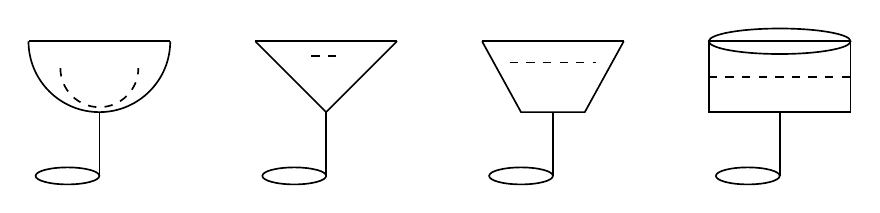
\begin{tikzpicture}[scale=0.9, semithick,
  every node/.style={inner sep=1pt}]

  % ---------------- 半球形杯 ----------------
  \begin{scope}[shift={(0,0)}]
    \draw (-1,3) arc[start angle=180,end angle=360,radius=1];
    \draw (-1,3) -- (-1,3);
    \draw (-1,3) -- (1,3);
    \draw[dashed] (-0.55,2.62) arc[start angle=180,end angle=360,radius=0.55];
    \draw (0,2) -- (0,1.1);
    \draw (-0.45,1.1) ellipse (0.45 and 0.12);
  \end{scope}

  % ---------------- 圆锥形杯 ----------------
  \begin{scope}[shift={(3.2,0)}]
    \draw (-1,3) -- (0,2) -- (1,3);
    \draw (-1,3) -- (1,3);
    \draw[dashed] (-0.21,2.79) -- (0.21,2.79);
    \draw (0,2) -- (0,1.1);
    \draw (-0.45,1.1) ellipse (0.45 and 0.12);
  \end{scope}

  % ---------------- 圆台形杯 ----------------
  \begin{scope}[shift={(6.4,0)}]
    \draw (-1,3) -- (-0.45,2) -- (0.45,2) -- (1,3);
    \draw (-1,3) -- (1,3);
    \draw[dashed] (-0.61,2.7) -- (0.61,2.7);
    \draw (0,2) -- (0,1.1);
    \draw (-0.45,1.1) ellipse (0.45 and 0.12);
  \end{scope}

  % ---------------- 圆柱形杯 ----------------
  \begin{scope}[shift={(9.6,0)}]
    \draw (-1,3) -- (1,3) -- (1,2) -- (-1,2) -- cycle;
    \draw (0,3) ellipse (1 and 0.18);
    \draw[dashed] (-1,2.5) -- (1,2.5);
    \draw (0,2) -- (0,1.1);
    \draw (-0.45,1.1) ellipse (0.45 and 0.12);
  \end{scope}
\end{tikzpicture}
\end{center}
\nopagebreak[4]
（A）$h_2>h_1>h_4$

（B）$h_1>h_2>h_3$

（C）$h_3>h_2>h_4$

（D）$h_2>h_4>h_1$

\Needspace{4\baselineskip}
\textbf{解析}

设杯高为 $H$，杯口半径为 $R$。

\begin{itemize}
\item 圆柱形杯（$h_4$）：体积与高度成正比，半杯时 $h_4=\dfrac H2$；
\item 圆锥形杯（$h_2$）：体积 $\propto h^3$，半杯时 $h_2=\dfrac{H}{\sqrt[3]{2}}\approx0.794H$；
\item 半球形杯（$h_1$）：由球缺体积公式，半杯时 $h_1\approx0.66H$。
\end{itemize}

故 $h_2>h_1>h_4$，选 A。（圆台杯底半径小于口半径，半杯时高度最低，约 $0.39H$；四个选项中只有 A 与 $h_2>h_1>h_4$ 一致。）

\gkanswer{答案：A。}

\end{answer}
\begin{answer}
\gksolhead{12}{}

\textbf{题目}：

设椭圆 $\dfrac{x^2}{a^2}+\dfrac{y^2}{b^2}=1$（$a>b>0$）的离心率为 $e=\dfrac12$，右焦点为 $F(c,0)$，方程 $ax^2+bx-c=0$ 的两个实根分别为 $x_1$ 和 $x_2$，则点 $P(x_1,x_2)$（　）

（A）必在圆 $x^2+y^2=2$ 上

（B）必在圆 $x^2+y^2=2$ 外

（C）必在圆 $x^2+y^2=2$ 内

（D）以上三种情形都有可能

\Needspace{4\baselineskip}
\textbf{解析}

\Needspace{5\baselineskip}
由 $e=\dfrac12$ 得 $a=2c$，$b^2=a^2-c^2=3c^2$，故 $b=\sqrt3c$。方程

\nopagebreak[4]
\[2cx^2+\sqrt3cx-c=0\]

\Needspace{5\baselineskip}
两边除以 $c$：

\nopagebreak[4]
\[2x^2+\sqrt3x-1=0.\]

\Needspace{5\baselineskip}
设两根为 $x_1$，$x_2$，由韦达定理，

\nopagebreak[4]
\[x_1+x_2=-\frac{\sqrt3}{2},\qquad x_1x_2=-\frac12.\]

\Needspace{5\baselineskip}
于是

\nopagebreak[4]
\[x_1^2+x_2^2=(x_1+x_2)^2-2x_1x_2=\frac34+1=\frac74<2.\]

故点 $P(x_1,x_2)$ 必在圆 $x^2+y^2=2$ 内。

\gkanswer{答案：C。}

\end{answer}
\begin{answer}
\gksolhead{13}{}

\textbf{题目}：

在平面直角坐标系中，正方形 $OABC$ 的对角线 $OB$ 的两端点分别为 $O(0,0)$，$B(1,1)$，则 $\overrightarrow{AB}\cdot\overrightarrow{AC}=$\gkblank{}。

\Needspace{4\baselineskip}
\textbf{解析}

\Needspace{5\baselineskip}
正方形 $OABC$ 以 $OB$ 为对角线，取

\nopagebreak[4]
\[A(1,0),\qquad C(0,1),\]

\Needspace{5\baselineskip}
则 $B(1,1)$，且

\nopagebreak[4]
\[\overrightarrow{AB}=(0,1),\qquad \overrightarrow{AC}=(-1,1),\]

\nopagebreak[4]
\[\overrightarrow{AB}\cdot\overrightarrow{AC}=0\times(-1)+1\times1=1.\]

（若交换 $A$，$C$，结果相同。）

\gkanswer{答案：$1$。}

\end{answer}
\begin{answer}
\gksolhead{14}{}

\textbf{题目}：

已知等差数列 $\{a_n\}$ 的前 $n$ 项和为 $S_n$，若 $S_{12}=21$，则 $a_2+a_5+a_8+a_{11}=$\gkblank{}。

\Needspace{4\baselineskip}
\textbf{解析}

\nopagebreak[4]
\[S_{12}=\frac{12(a_1+a_{12})}{2}=6(a_1+a_{12})=21,\]

故 $a_1+a_{12}=\dfrac72$。

\Needspace{5\baselineskip}
又

\nopagebreak[4]
\[a_2+a_{11}=a_5+a_8=a_1+a_{12},\]

\Needspace{5\baselineskip}
故

\nopagebreak[4]
\[a_2+a_5+a_8+a_{11}=2(a_1+a_{12})=7.\]

\gkanswer{答案：$7$。}

\end{answer}
\begin{answer}
\gksolhead{15}{}

\textbf{题目}：

已知函数 $y=f(x)$ 存在反函数 $y=f^{-1}(x)$，若函数 $y=f(1+x)$ 的图象经过点 $(3,1)$，则函数 $y=f^{-1}(x)$ 的图象必经过点\gkblank{}。

\Needspace{4\baselineskip}
\textbf{解析}

\Needspace{5\baselineskip}
$y=f(1+x)$ 的图象过 $(3,1)$，即

\nopagebreak[4]
\[f(1+3)=f(4)=1.\]

故 $f^{-1}(1)=4$，即 $y=f^{-1}(x)$ 的图象过点 $(1,4)$。

\gkanswer{答案：$(1,4)$。}

\end{answer}
\begin{answer}
\gksolhead{16}{}

\textbf{题目}：

如图，正方体 $AC_1$ 的棱长为 $1$，过点 $A$ 作平面 $A_1BD$ 的垂线，垂足为点 $H$。有下列四个命题：

A. 点 $H$ 是 $\triangle A_1BD$ 的垂心；

B. $AH$ 垂直平面 $CB_1D_1$；

C. 二面角 $C-B_1D_1-C_1$ 的正切值为 $\sqrt2$；

D. 点 $H$ 到平面 $A_1B_1C_1D_1$ 的距离为 $\dfrac34$。

其中真命题的代号是\gkblank{}。（写出所有真命题的代号）
\nopagebreak[4]
\begin{center}% 2007 年江西卷文科第 16 题：棱长为 1 的正方体 AC1，AH⊥平面 A1BD，H 为垂足。
%   图中标出 A、B、C、D、A1、B1、C1、D1、H 与平面 A1BD。
% 来源 PDF：gaokaomath-src/普通高考/2007/2007江西文.pdf
% SHA-256：6602cbc393b02e9940beb0035be6e2a28d88a77e0e7792260dcd4c873b542a82
% 原页：2007江西文.pdf 第 1 页（A3 三栏）第 3 栏，书页码 387。
% 重绘依据：按原页正方体斜投影、平面 A1BD 与垂足 H 的位置重绘。
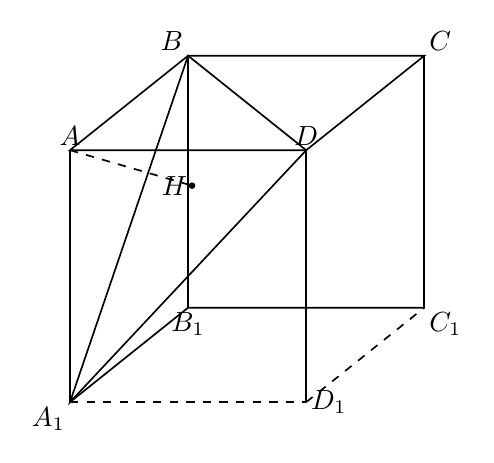
\begin{tikzpicture}[scale=1.0, semithick,
  every node/.style={inner sep=1.5pt}]

  \coordinate (A)  at (0,3.2);
  \coordinate (B)  at (1.5,4.4);
  \coordinate (C)  at (4.5,4.4);
  \coordinate (D)  at (3.0,3.2);
  \coordinate (A1) at (0,0);
  \coordinate (B1) at (1.5,1.2);
  \coordinate (C1) at (4.5,1.2);
  \coordinate (D1) at (3.0,0);

  % 被遮挡的棱
  \draw[dashed] (A1) -- (D1);
  \draw[dashed] (D1) -- (C1);
  \draw[dashed] (D1) -- (D);

  % 可见的棱
  \draw (A) -- (B) -- (C) -- (D) -- cycle;
  \draw (A) -- (A1);
  \draw (B) -- (B1);
  \draw (C) -- (C1);
  \draw (D) -- (D1);
  \draw (A1) -- (B1) -- (C1);

  % 平面 A1BD 与垂足 H
  \draw (A1) -- (B) -- (D) -- cycle;
  \coordinate (H) at (1.55,2.75);
  \draw[dashed] (A) -- (H);
  \fill (H) circle (1.2pt);

  \node[above] at (A) {$A$};
  \node[above left] at (B) {$B$};
  \node[above right] at (C) {$C$};
  \node[above] at (D) {$D$};
  \node[below left] at (A1) {$A_1$};
  \node[below] at (B1) {$B_1$};
  \node[below right] at (C1) {$C_1$};
  \node[right] at (D1) {$D_1$};
  \node[left] at (H) {$H$};
\end{tikzpicture}
\end{center}
\nopagebreak[4]
\Needspace{4\baselineskip}
\textbf{解析}

\Needspace{5\baselineskip}
以 $A$ 为原点，$AB$，$AD$，$AA_1$ 为 $x$，$y$，$z$ 轴建立坐标系，棱长为 $1$：

\nopagebreak[4]
\[A(0,0,0),\ B(1,0,0),\ D(0,1,0),\ A_1(0,0,1),\]

\nopagebreak[4]
\[C(1,1,0),\ B_1(1,0,1),\ C_1(1,1,1),\ D_1(0,1,1).\]

\Needspace{5\baselineskip}
平面 $A_1BD$ 的方程为

\nopagebreak[4]
\[x+y+z=1,\]

\Needspace{5\baselineskip}
法向量 $\boldsymbol n=(1,1,1)$。$AH$ 沿 $\boldsymbol n$ 方向，$H$ 为 $t(1,1,1)$ 与平面的交点，$3t=1$，故

\nopagebreak[4]
\[H\left(\frac13,\frac13,\frac13\right).\]

A：$\triangle A_1BD$ 为等边三角形，$H$ 到 $A_1$，$B$，$D$ 距离相等，且 $AH$ 垂直于平面，故 $H$ 为外心，也是垂心，正确。

B：平面 $CB_1D_1$ 的方程也为 $x+y+z=2$，法向量同为 $(1,1,1)$，与 $AH$ 平行，故 $AH\perp$ 平面 $CB_1D_1$，正确。

\Needspace{5\baselineskip}
C：平面 $CB_1D_1$ 的法向量 $\boldsymbol n_1=(1,1,1)$，平面 $B_1D_1C_1$（即上底面）的法向量 $\boldsymbol n_2=(0,0,1)$。二面角 $\theta$ 满足

\nopagebreak[4]
\[\cos\theta=\frac{|\boldsymbol n_1\cdot\boldsymbol n_2|}{|\boldsymbol n_1||\boldsymbol n_2|}=\frac1{\sqrt3},\]

\Needspace{5\baselineskip}
故

\nopagebreak[4]
\[\tan\theta=\sqrt{3-1}=\sqrt2,\]

正确。

\Needspace{5\baselineskip}
D：$H$ 到平面 $A_1B_1C_1D_1$（$z=1$）的距离为

\nopagebreak[4]
\[1-\frac13=\frac23\neq\frac34,\]

错误。

故真命题为 A、B、C。

\gkanswer{答案：A、B、C。}

\end{answer}
\begin{answer}
\gksolhead{17}{}

\textbf{题目}：

\Needspace{5\baselineskip}
已知函数

\nopagebreak[4]
\[f(x)=\begin{cases}cx+1,&0<x<c,\\ 2^{-\frac{x}{c^2}}+1,&c\leqslant x<1,\end{cases}\]

在区间 $(0,1)$ 内连续，且 $f(c^2)=\dfrac98$。

（1）求常数 $c$ 的值；

（2）解不等式 $f(x)>\dfrac{\sqrt2}{8}+1$。

\Needspace{4\baselineskip}
\textbf{解析}

\Needspace{5\baselineskip}
（1）$f(x)$ 在 $(0,1)$ 内连续，故在 $x=c$ 处连续：

\nopagebreak[4]
\[\lim_{x\to c^-}f(x)=c\cdot c+1=c^2+1,\]

\nopagebreak[4]
\[\lim_{x\to c^+}f(x)=2^{-\frac{c}{c^2}}+1=2^{-\frac1c}+1.\]

\Needspace{5\baselineskip}
于是

\nopagebreak[4]
\[c^2=2^{-\frac1c}.\]

\Needspace{5\baselineskip}
又 $c^2<c$（因 $0<c<1$），故 $f(c^2)$ 用第一段：

\nopagebreak[4]
\[f(c^2)=c\cdot c^2+1=c^3+1=\frac98,\]

\nopagebreak[4]
\[c^3=\frac18\ \Rightarrow\ c=\frac12.\]

检验：$c^2=\dfrac14$，$2^{-1/c}=2^{-2}=\dfrac14$，连续条件成立。

\Needspace{5\baselineskip}
（2）$c=\dfrac12$，故

\nopagebreak[4]
\[f(x)=\begin{cases}\dfrac12x+1,&0<x<\dfrac12,\\ 2^{-4x}+1,&\dfrac12\leqslant x<1.\end{cases}\]

不等式 $f(x)>\dfrac{\sqrt2}{8}+1$。

\Needspace{5\baselineskip}
当 $0<x<\dfrac12$：

\nopagebreak[4]
\[\frac12x+1>1+\frac{\sqrt2}{8}\ \Rightarrow\ x>\frac{\sqrt2}{4}.\]

故 $\dfrac{\sqrt2}{4}<x<\dfrac12$。

\Needspace{5\baselineskip}
当 $\dfrac12\leqslant x<1$：

\nopagebreak[4]
\[2^{-4x}+1>1+\frac{\sqrt2}{8}.\]

\Needspace{5\baselineskip}
注意 $\dfrac{\sqrt2}{8}=2^{-5/2}$，故

\nopagebreak[4]
\[2^{-4x}>2^{-5/2}\ \Rightarrow\ -4x>-\frac52\ \Rightarrow\ x<\frac58.\]

故 $\dfrac12\leqslant x<\dfrac58$。

\Needspace{5\baselineskip}
合并得

\nopagebreak[4]
\[\frac{\sqrt2}{4}<x<\frac58.\]

\gkanswer{答案：（1）$c=\dfrac12$；（2）$\left(\dfrac{\sqrt2}{4},\dfrac58\right)$。}

\end{answer}
\begin{answer}
\gksolhead{18}{}

\textbf{题目}：

如图，函数 $y=2\cos(\omega x+\theta)$（$x\in\mathbf R$，$0\leqslant\theta\leqslant\dfrac{\pi}{2}$）的图象与 $y$ 轴交于点 $(0,\sqrt3)$，且在该点处切线的斜率为 $-2$。

（1）求 $\theta$ 和 $\omega$ 的值；

（2）已知点 $A\left(\dfrac{\pi}{2},0\right)$，点 $P$ 是该函数图象上的一点，点 $Q(x_0,y_0)$ 是 $PA$ 的中点，当 $y_0=\dfrac{\sqrt3}{2}$，$x_0\in\left[\dfrac{\pi}{2},\pi\right]$ 时，求 $x_0$ 的值。
\nopagebreak[4]
\begin{center}% 2007 年江西卷文科第 18 题：y=2cos(ωx+θ) 的图象、点 A(π/2,0)、P 与 PA 中点 Q。
%   图中按 θ=π/6、ω=2 及 Q=(2π/3,√3/2)、P=(5π/6,√3) 的示意位置绘制。
% 来源 PDF：gaokaomath-src/普通高考/2007/2007江西文.pdf
% SHA-256：6602cbc393b02e9940beb0035be6e2a28d88a77e0e7792260dcd4c873b542a82
% 原页：2007江西文.pdf 第 1 页（A3 三栏）第 3 栏，书页码 387。
% 重绘依据：按原页余弦曲线、A、P、Q 的相对位置重绘。
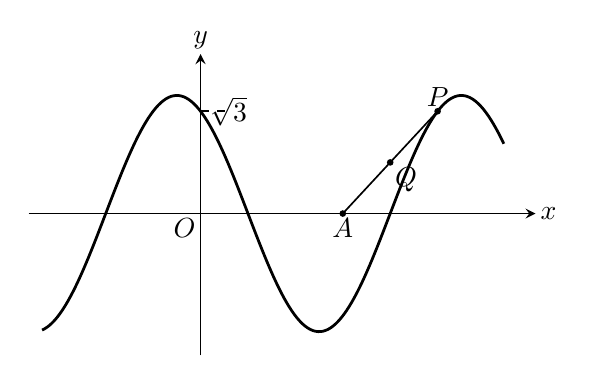
\begin{tikzpicture}[x=1.15cm, y=0.75cm, semithick,
  every node/.style={inner sep=1.5pt}]

  \draw[->,>=stealth] (-1.9,0) -- (3.7,0) node[right] {$x$};
  \draw[->,>=stealth] (0,-2.4) -- (0,2.7) node[above] {$y$};
  \node[below left] at (0,0) {$O$};

  \draw[domain=-1.75:3.35,samples=180,line width=1pt]
    plot (\x,{2*cos(deg(2*\x + pi/6))});

  \coordinate (A) at (1.5708,0);
  \coordinate (Q) at (2.0944,0.8660);
  \coordinate (P) at (2.6180,1.7320);

  \draw (A) -- (P);
  \fill (A) circle (1.2pt);
  \fill (Q) circle (1.2pt);
  \fill (P) circle (1.2pt);
  \node[below] at (A) {$A$};
  \node[below right] at (Q) {$Q$};
  \node[above] at (P) {$P$};

  % y 轴上的 √3 标记
  \draw[dashed] (0,1.732) -- (0.35,1.732);
  \node[right] at (0.05,1.732) {$\sqrt3$};
\end{tikzpicture}
\end{center}
\nopagebreak[4]
\Needspace{4\baselineskip}
\textbf{解析}

\Needspace{5\baselineskip}
（1）$x=0$ 时 $y=2\cos\theta=\sqrt3$，故

\nopagebreak[4]
\[\cos\theta=\frac{\sqrt3}{2}.\]

\Needspace{5\baselineskip}
又 $0\leqslant\theta\leqslant\dfrac{\pi}{2}$，故

\nopagebreak[4]
\[\theta=\frac{\pi}{6}.\]

\Needspace{5\baselineskip}
求导：

\nopagebreak[4]
\[y'=-2\omega\sin(\omega x+\theta).\]

\Needspace{5\baselineskip}
在 $x=0$ 处斜率为

\nopagebreak[4]
\[-2\omega\sin\theta=-2\omega\cdot\frac12=-\omega=-2,\]

\Needspace{5\baselineskip}
故

\nopagebreak[4]
\[\omega=2.\]

\Needspace{5\baselineskip}
（2）由（1），

\nopagebreak[4]
\[y=2\cos\left(2x+\frac{\pi}{6}\right).\]

\Needspace{5\baselineskip}
设 $P(x_P,y_P)$。$Q(x_0,y_0)$ 为 $PA$ 中点，$A\left(\dfrac{\pi}{2},0\right)$，故

\nopagebreak[4]
\[x_P=2x_0-\frac{\pi}{2},\qquad y_P=2y_0-0=\sqrt3.\]

\Needspace{5\baselineskip}
$P$ 在图象上：

\nopagebreak[4]
\[2\cos\left(2x_P+\frac{\pi}{6}\right)=\sqrt3,\]

\Needspace{5\baselineskip}
即

\nopagebreak[4]
\[\cos\left(2\left(2x_0-\frac{\pi}{2}\right)+\frac{\pi}{6}\right)=\frac{\sqrt3}{2},\]

\nopagebreak[4]
\[\cos\left(4x_0-\frac{5\pi}{6}\right)=\frac{\sqrt3}{2}.\]

\Needspace{5\baselineskip}
故

\nopagebreak[4]
\[4x_0-\frac{5\pi}{6}=\pm\frac{\pi}{6}+2k\pi.\]

\Needspace{5\baselineskip}
若取 $+\dfrac{\pi}{6}$：

\nopagebreak[4]
\[4x_0=\pi+2k\pi\ \Rightarrow\ x_0=\frac{\pi}{4}+\frac{k\pi}{2}.\]

\Needspace{5\baselineskip}
在 $\left[\dfrac{\pi}{2},\pi\right]$ 内取 $k=1$，得

\nopagebreak[4]
\[x_0=\frac{3\pi}{4}.\]

\Needspace{5\baselineskip}
若取 $-\dfrac{\pi}{6}$：

\nopagebreak[4]
\[4x_0=\frac{2\pi}{3}+2k\pi\ \Rightarrow\ x_0=\frac{\pi}{6}+\frac{k\pi}{2}.\]

\Needspace{5\baselineskip}
在 $\left[\dfrac{\pi}{2},\pi\right]$ 内取 $k=1$，得

\nopagebreak[4]
\[x_0=\frac{2\pi}{3}.\]

\Needspace{5\baselineskip}
故

\nopagebreak[4]
\[x_0=\frac{2\pi}{3}\ \text{\text{或}}\ \frac{3\pi}{4}.\]

\gkanswer{答案：（1）$\theta=\dfrac{\pi}{6}$，$\omega=2$；（2）$x_0=\dfrac{2\pi}{3}$ 或 $\dfrac{3\pi}{4}$。}

\end{answer}
\begin{answer}
\gksolhead{19}{}

\textbf{题目}：

栽培甲、乙两种果树，先要培育成苗，然后再进行移栽。已知甲、乙两种果树成苗的概率分别为 $0.6$，$0.5$，移栽后成活的概率分别为 $0.7$，$0.9$。

（1）求甲、乙两种果树至少有一种果树成苗的概率；

（2）求恰好一种果树能栽培成苗且移栽成活的概率。

\Needspace{4\baselineskip}
\textbf{解析}

\Needspace{5\baselineskip}
（1）甲、乙都不成苗的概率为

\nopagebreak[4]
\[(1-0.6)(1-0.5)=0.4\times0.5=0.2,\]

\Needspace{5\baselineskip}
故至少一种成苗的概率为

\nopagebreak[4]
\[1-0.2=0.8.\]

\Needspace{5\baselineskip}
（2）一种果树“栽培成苗且移栽成活”的概率为成苗率与成活率之积：

\nopagebreak[4]
\[p_{\text{\text{甲}}}=0.6\times0.7=0.42,\qquad p_{\text{\text{乙}}}=0.5\times0.9=0.45.\]

\Needspace{5\baselineskip}
恰好一种成功的概率为

\nopagebreak[4]
\[0.42(1-0.45)+(1-0.42)\times0.45=0.42\times0.55+0.58\times0.45=0.231+0.261=0.492.\]

\gkanswer{答案：（1）$0.8$；（2）$0.492$。}

\end{answer}
\begin{answer}
\gksolhead{20}{}

\textbf{题目}：

如图是一个直三棱柱（以 $A_1B_1C_1$ 为底面）被一平面所截得到的几何体，截面为 $ABC$。已知 $A_1B_1=B_1C_1=1$，$\angle A_1B_1C_1=90^\circ$，$AA_1=4$，$BB_1=2$，$CC_1=3$。

（1）设点 $O$ 是 $AB$ 的中点，证明：$OC\parallel$ 平面 $A_1B_1C_1$；

（2）求 $AB$ 与平面 $AA_1C_1C$ 所成的角的大小；

（3）求此几何体的体积。
\nopagebreak[4]
\begin{center}% 2007 年江西卷文科第 20 题：直三棱柱被平面 ABC 截得的几何体。
%   底面 A1B1C1 为等腰直角三角形，AA1=4、BB1=2、CC1=3；O 为 AB 中点。
% 来源 PDF：gaokaomath-src/普通高考/2007/2007江西文.pdf
% SHA-256：6602cbc393b02e9940beb0035be6e2a28d88a77e0e7792260dcd4c873b542a82
% 原页：2007江西文.pdf 第 2 页（A3 三栏）第 1 栏，书页码 388。
% 重绘依据：按原页截棱柱的斜投影与 O、C 的位置重绘。
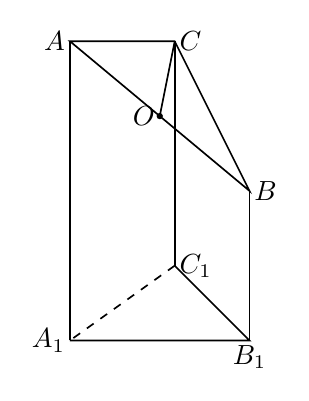
\begin{tikzpicture}[scale=0.95, semithick,
  every node/.style={inner sep=1.5pt}]

  \coordinate (A1) at (0,0);
  \coordinate (B1) at (2.4,0);
  \coordinate (C1) at (1.4,1.0);
  \coordinate (A)  at (0,4.0);
  \coordinate (B)  at (2.4,2.0);
  \coordinate (C)  at (1.4,4.0);
  \coordinate (O)  at (1.2,3.0);

  % 底面
  \draw (A1) -- (B1) -- (C1);
  \draw[dashed] (C1) -- (A1);
  % 侧棱
  \draw (A1) -- (A);
  \draw (B1) -- (B);
  \draw (C1) -- (C);
  % 截面 ABC
  \draw (A) -- (B) -- (C) -- cycle;
  % O 与 OC
  \fill (O) circle (1.2pt);
  \draw (O) -- (C);

  \node[left] at (A) {$A$};
  \node[right] at (B) {$B$};
  \node[right] at (C) {$C$};
  \node[left] at (A1) {$A_1$};
  \node[below] at (B1) {$B_1$};
  \node[right] at (C1) {$C_1$};
  \node[left] at (O) {$O$};
\end{tikzpicture}
\end{center}
\nopagebreak[4]
\Needspace{4\baselineskip}
\textbf{解析}

\Needspace{5\baselineskip}
以 $B_1$ 为原点，$B_1A_1$，$B_1C_1$，$B_1B$ 所在直线分别为 $x$，$y$，$z$ 轴建立坐标系：

\nopagebreak[4]
\[A_1(1,0,0),\ B_1(0,0,0),\ C_1(0,1,0),\]

\nopagebreak[4]
\[A(1,0,4),\ B(0,0,2),\ C(0,1,3).\]

\Needspace{5\baselineskip}
（1）$O$ 为 $AB$ 中点：

\nopagebreak[4]
\[O\left(\frac12,0,3\right).\]

\nopagebreak[4]
\[\overrightarrow{OC}=\left(-\frac12,1,0\right).\]

\Needspace{5\baselineskip}
平面 $A_1B_1C_1$ 为 $z=0$，其法向量为 $(0,0,1)$，且

\nopagebreak[4]
\[\overrightarrow{OC}\cdot(0,0,1)=0,\]

故 $OC$ 平行于平面 $A_1B_1C_1$。又 $O\notin$ 平面 $A_1B_1C_1$，所以 $OC\parallel$ 平面 $A_1B_1C_1$。

\Needspace{5\baselineskip}
（2）$\overrightarrow{AB}=(-1,0,-2)$。平面 $AA_1C_1C$ 过 $A(1,0,4)$，$A_1(1,0,0)$，$C(0,1,3)$，其方程为

\nopagebreak[4]
\[x+y=1,\]

\Needspace{5\baselineskip}
法向量 $\boldsymbol n=(1,1,0)$。设 $AB$ 与平面所成角为 $\varphi$，则

\nopagebreak[4]
\[\sin\varphi=\frac{|\overrightarrow{AB}\cdot\boldsymbol n|}{|\overrightarrow{AB}||\boldsymbol n|}=\frac{|-1|}{\sqrt5\cdot\sqrt2}=\frac1{\sqrt{10}}.\]

\Needspace{5\baselineskip}
故

\nopagebreak[4]
\[\tan\varphi=\frac1{\sqrt{10-1}}=\frac13,\]

\nopagebreak[4]
\[\varphi=\arctan\frac13.\]

\Needspace{5\baselineskip}
（3）底面 $A_1B_1C_1$ 是直角边为 $1$ 的等腰直角三角形，面积

\nopagebreak[4]
\[S=\frac12\times1\times1=\frac12.\]

\Needspace{5\baselineskip}
截面 $ABC$ 所在平面过 $A(1,0,4)$，$B(0,0,2)$，$C(0,1,3)$，其方程为

\nopagebreak[4]
\[z=2x+y+2.\]

\Needspace{5\baselineskip}
底面重心为 $\left(\dfrac13,\dfrac13,0\right)$，该处高为

\nopagebreak[4]
\[h=2\times\frac13+\frac13+2=3.\]

\Needspace{5\baselineskip}
故体积

\nopagebreak[4]
\[V=Sh=\frac12\times3=\frac32.\]

\gkanswer{答案：（1）证明见解析；（2）$\arctan\dfrac13$；（3）$\dfrac32$。}

\end{answer}
\begin{answer}
\gksolhead{21}{}

\textbf{题目}：

设 $\{a_n\}$ 为等比数列，$a_1=1$，$a_2=3$。

（1）求最小的自然数 $n$，使 $a_n\geqslant2007$；

（2）求和：$T_{2n}=\dfrac1{a_1}-\dfrac2{a_2}+\dfrac3{a_3}-\cdots-\dfrac{2n}{a_{2n}}$。

\Needspace{4\baselineskip}
\textbf{解析}

\Needspace{5\baselineskip}
（1）等比数列公比 $q=\dfrac{a_2}{a_1}=3$，故

\nopagebreak[4]
\[a_n=3^{n-1}.\]

\Needspace{5\baselineskip}
要求 $3^{n-1}\geqslant2007$。因为

\nopagebreak[4]
\[3^6=729<2007<2187=3^7,\]

故 $n-1=7$，最小 $n=8$。

\Needspace{5\baselineskip}
（2）设

\nopagebreak[4]
\[T_{2n}=\sum_{k=1}^{2n}(-1)^{k-1}\frac{k}{a_k}=\sum_{k=1}^{2n}(-1)^{k-1}k\left(\frac13\right)^{k-1}.\]

\Needspace{5\baselineskip}
记 $x=-\dfrac13$，则

\nopagebreak[4]
\[T_{2n}=\sum_{k=1}^{2n}k x^{k-1}.\]

\Needspace{5\baselineskip}
利用公式

\nopagebreak[4]
\[\sum_{k=1}^{m}k x^{k-1}=\frac{1-(m+1)x^m+m x^{m+1}}{(1-x)^2},\]

\Needspace{5\baselineskip}
取 $m=2n$，$x=-\dfrac13$：

\nopagebreak[4]
\[x^{2n}=\frac1{3^{2n}},\qquad x^{2n+1}=-\frac1{3^{2n+1}},\]

\nopagebreak[4]
\[1-x=\frac43,\qquad (1-x)^2=\frac{16}{9}.\]

\Needspace{5\baselineskip}
分子：

\nopagebreak[4]
\[1-(2n+1)\frac1{3^{2n}}-2n\frac1{3^{2n+1}}
=1-\frac{3(2n+1)+2n}{3^{2n+1}}
=1-\frac{8n+3}{3^{2n+1}}.\]

\Needspace{5\baselineskip}
故

\nopagebreak[4]
\[T_{2n}=\frac{9}{16}\left[1-\frac{8n+3}{3^{2n+1}}\right].\]

\gkanswer{答案：（1）$8$；（2）$T_{2n}=\dfrac9{16}\left[1-\dfrac{8n+3}{3^{2n+1}}\right]$。}

\end{answer}